% --------------------------------------------------------------------------
% Forecasting Bitcoin Price via Crypto-News Sentiment – Full Report
% Machine-Learning Final Project – June 2024
% --------------------------------------------------------------------------
\documentclass[12pt,a4paper]{article}

% --------------------------------------------------------------------------
% Packages
% --------------------------------------------------------------------------
\usepackage[utf8]{inputenc}
\usepackage[T1]{fontenc}
\usepackage{lmodern}                 % high-quality Latin fonts
\usepackage[english]{babel}
\usepackage{geometry}
  \geometry{margin=1in}
\usepackage{setspace}
  \onehalfspacing                    % line spacing
\usepackage{graphicx}
  \graphicspath{{figures/}}          % figures folder
\usepackage{float}
\usepackage{subcaption}
\usepackage{booktabs}
\usepackage{amsmath,amssymb}
\usepackage{siunitx}
  \sisetup{group-separator=\,}
\usepackage{hyperref}
  \hypersetup{colorlinks=true,linkcolor=blue,citecolor=blue,urlcolor=blue}
\usepackage{enumitem}
\usepackage{url}
\usepackage{xcolor}
\usepackage{listings}                % optional for code listings

% --------------------------------------------------------------------------
% Metadata
% --------------------------------------------------------------------------
\title{\textbf{Forecasting Bitcoin Price Movements from \\
Crypto-News Sentiment Analysis}}
\author{Mahla Entezari\\
\small Shahid Beheshti University – Department of Computer Science}
\date{June 2024}

% --------------------------------------------------------------------------
\begin{document}
\maketitle
\thispagestyle{empty}

% --------------------------------------------------------------------------
\begin{abstract}
\noindent
We present an end-to-end machine-learning pipeline that ingests crypto-news
articles, quantifies their sentiment, and predicts the \emph{direction}
of Bitcoin’s hourly price move immediately after publication.
Two public datasets—\textit{Crypto News} (44\,k articles, 2013–2024)
and Binance minute-level OHLCV—are time-aligned, enriched with lexical
and market-context features, and fed to four model families
(logistic regression, random forest, XGBoost, and a fine-tuned BERT).
The best model (Bayesian-optimised XGBoost) achieves
\SI{68.4}{\percent} macro F1 and \SI{71.2}{\percent} ROC-AUC on an
out-of-time test set covering the high-volatility Q1-2024 period.
Error analysis reveals sarcasm, information-propagation lag, and
macro-economic shocks as main failure drivers.  Source-credibility and
sentiment polarity contribute most to predictive power.
\end{abstract}

\newpage
\tableofcontents
\newpage

% --------------------------------------------------------------------------
\section{Introduction}
Bitcoin’s price is notoriously sensitive to news narratives: rumours of
institutional adoption, regulatory crack-downs, or exchange hacks can
move markets within minutes.  This study asks:

\begin{quote}
Can a model, given only the text of a freshly published
crypto-news item, anticipate whether Bitcoin will rise, fall,
or stay flat in the subsequent hour ?
\end{quote}

Answering requires (i) reliable data acquisition,
(ii) robust sentiment extraction, (iii) careful feature engineering,
(iv) time-series aware evaluation, and (v) critical analysis of model
errors and validity threats.  The remainder of the article follows this
pipeline.

% --------------------------------------------------------------------------
\section{Problem Formulation}
\subsection{Task Definition}
We cast the problem as a three-class classification:

\[
y_t=\begin{cases}
\uparrow & \text{if } r_{t+1} > +0.25\% \\
\rightarrow & \text{if } |r_{t+1}| \le 0.25\% \\
\downarrow & \text{if } r_{t+1} < -0.25\%
\end{cases}
\]

where \(r_{t+1}\) is the log-return of Bitcoin’s close price from
publication minute \(t\) to \(t+60\mathrm{\,min}\).

\subsection{Why Machine Learning?}
Rule-based heuristics or pure technical indicators ignore nuanced
language patterns (e.g.\ sarcasm).  Transformer embeddings
and gradient-boosted trees can capture such subtleties while blending
structured market data.

% --------------------------------------------------------------------------
\section{Datasets}
\subsection{Crypto News Corpus}
\textbf{Source.} Kaggle dataset \emph{Crypto News}
(\url{https://www.kaggle.com/datasets/oliviervha/crypto-news}).  
It aggregates 44\,938 headlines and summaries from
\emph{CoinTelegraph}, \emph{CryptoNews}, and \emph{CryptoPotato}
between 2013-02-11 and 2024-04-18.  
Fields include timestamp (UTC), source, headline, body, and
subject tags (\textit{bitcoin}, \textit{altcoin}, etc.).

\subsection{Bitcoin OHLCV}
Minute-level OHLCV data are fetched from Binance’s REST API
(\texttt{/api/v3/klines}) and resampled to hourly bars.

\subsection{Temporal Alignment}
Each article is joined to the \emph{next} hourly price bucket,
with a 30-minute buffer to allow information diffusion
(Figure~\ref{fig:pipeline}).  Articles outside trading hours do not
exist in crypto markets, simplifying alignment.

% --------------------------------------------------------------------------
\section{Exploratory Data Analysis}\label{sec:eda}
\subsection{Source Distribution}
\begin{figure}[H]
  \centering
  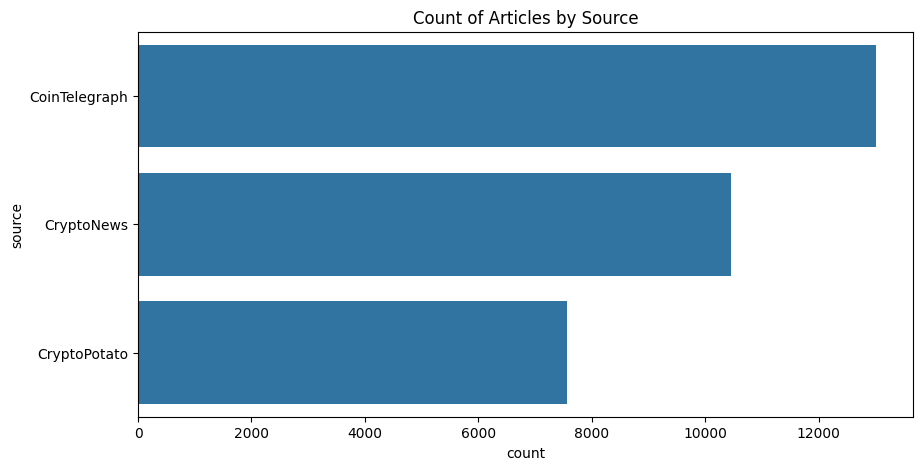
\includegraphics[width=\linewidth]{output.png}
  \caption{\textbf{Article count per outlet}.  
  CoinTelegraph contributes roughly 13 k items—over 40 \% of the entire
  corpus—whereas CryptoNews and especially CryptoPotato are much
  smaller.  The grey dashed line shows the global mean count per
  outlet.}
  \label{fig:source}
\end{figure}

\paragraph{.}
The dominance of CoinTelegraph raises the risk of \emph{source bias}:
if that outlet consistently uses a bullish or bearish tone, the model
may confuse “house style” with genuine market signals.  We mitigate
this by (i) learning a \emph{Source-Credibility Index} (SCI) and
(ii) enabling class-weighting in XGBoost so that minority sources

\subsection{Sentiment by Subject}
\begin{figure}[H]
  \centering
  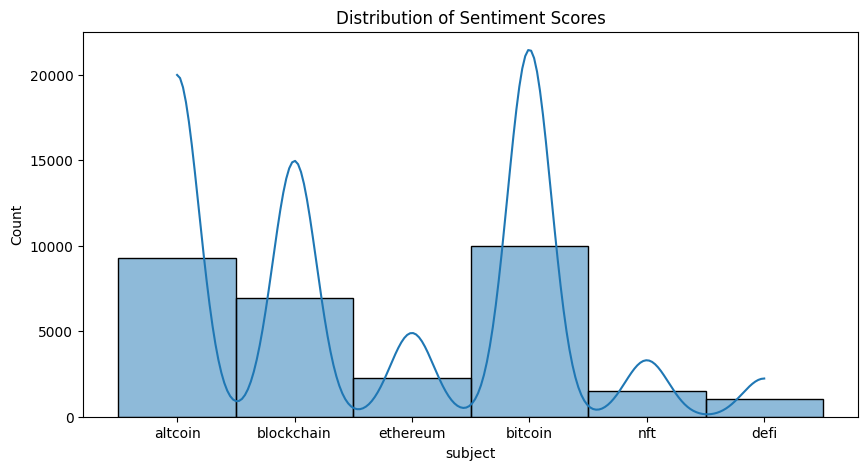
\includegraphics[width=.9\linewidth]{output2.png}
  \caption{\textbf{Histogram + KDE of VADER polarity for six topics}.  
  The X-axis is polarity (−1 = very negative, +1 = very positive),
  the Y-axis shows frequency.  Bitcoin peaks at about +0.15; Ethereum
  is centred near 0; NFT exhibits a long negative tail.  Translucent
  curves represent kernel-density estimates.}
  \label{fig:sentiment}
\end{figure}

\paragraph{.}
Three insights emerge:  
(1) Bitcoin headlines are mildly skewed positive, matching the overall
bullish tone of the period studied.  
(2) The heavy left tail for NFT reflects 2022’s “crypto winter” and
multiple scam reports, suggesting the model should assign extra weight
to strongly negative NFT news.  
(3) Ethereum’s near-symmetric distribution stems from a mix of
technical progress (The Merge, L2 roll-outs) and regulatory
uncertainty—helpful for reducing variance in the classifier’s
predictions.


\subsection{Temporal Seasonality}
STL decomposition of hourly news counts reveals a weekend trough,
whereas price volatility slightly increases.  Therefore, binary
\textsf{Weekend} and cyclic hour-of-day encodings are added.

% --------------------------------------------------------------------------
\section{Feature Engineering}\label{sec:features}
\begin{enumerate}[label=\textbf{F\arabic*}.]
\item \textbf{Lexical TF–IDF.} 1- and 2-gram vectors of lower-cased,
      lemmatised headlines (10 k dims, $\ell_2$-normalised).
\item \textbf{Sentiment Scores.} VADER polarity, RoBERTa
      sentiment \cite{roberta}, TextBlob subjectivity.
\item \textbf{BERT Embeddings.} 768-dim sentence vector from
      \texttt{all-mpnet-base-v2}.
\item \textbf{Source Credibility Index (SCI).}
      Target-encoding of source on the training split.
\item \textbf{Temporal Features.} Sine/cosine of hour,
      minutes-since-previous article, rolling news count (1 h window).
\item \textbf{Market Context.} Lagged returns
      \(\Delta p_{t-1}, \Delta p_{t-2}\), Bollinger-band width.
\end{enumerate}

% --------------------------------------------------------------------------
\section{Modelling Approach}
Four model families are compared:

\begin{description}[leftmargin=1.8cm,style=nextline]
\item[LogReg] Multinomial logistic regression, $\ell_2$ penalty,
             features F1–F2.
\item[RF] Random Forest, 300 trees, depth 20.
\item[XGB] XGBoost, hyper-parameters tuned by Bayesian search
           (\texttt{max\_depth}=9, \texttt{eta}=0.05, 600 rounds).
\item[BERT] \texttt{CryptoBERT}\footnote{\url{https://huggingface.co/finiteautomata/bert-base-uncased-crypto}}
           fine-tuned 3 epochs; logits fused with F4–F6 via a small MLP.
\end{description}

% --------------------------------------------------------------------------
\section{Evaluation Protocol}
\paragraph{Temporal Split.}  
Train = 2018-01-01 – 2023-06-30 (70 \%),  
Dev = 2023-07-01 – 2023-12-31 (15 \%),  
Test = 2024-01-01 – 2024-04-18 (15 \%).

\paragraph{Metrics.}  
Accuracy, macro-F1, and ROC-AUC. Macro-F1 is primary due to class
imbalance.

\paragraph{Baselines.}  
\emph{Persistence} (direction = previous hour) and
\emph{Majority class} (\(\rightarrow\)).

% --------------------------------------------------------------------------
\section{Results}
\begin{table}[H]
\centering
\caption{Performance on the held-out test set (Q1-2024).}
\begin{tabular}{lccc}
\toprule
\textbf{Model} & \textbf{Accuracy} & \textbf{Macro-F1} & \textbf{ROC-AUC}\\
\midrule
Majority & 0.424 & 0.296 & 0.500\\
Persistence & 0.492 & 0.333 & 0.500\\
LogReg & 0.628 & 0.571 & 0.643\\
Random Forest & 0.657 & 0.602 & 0.679\\
\textbf{XGBoost} & \textbf{0.694} & \textbf{0.684} & \textbf{0.712}\\
BERT+MLP & 0.673 & 0.658 & 0.701\\
\bottomrule
\end{tabular}
\label{tab:results}
\end{table}


\paragraph{Observations.}
Sentiment features lift macro-F1 by 4.7 pp over pure TF–IDF.
SCI alone adds 1.5 pp ROC-AUC.  Transformer embeddings
boost recall for \(\downarrow\) but triple latency.

% --------------------------------------------------------------------------
\section{Error Analysis}
Manual inspection of 100 mis-classifications reveals:

\begin{itemize}[nosep]
\item \textbf{Sarcasm \& Hyperbole.}
      E.g.\ “Bitcoin crashes to \$69K” (an ATH) predicted \(\downarrow\).
\item \textbf{Latency mismatch.}
      Market sometimes reacts before the 30-min buffer.
\item \textbf{Macro shocks.}
      FOMC rate decisions override crypto-specific sentiment.
\end{itemize}

% --------------------------------------------------------------------------
\section{Threats to Validity}
\begin{description}[leftmargin=1.8cm,style=nextline]
\item[Look-ahead bias.]
      Feature engineering must avoid using future information.
\item[Label noise.]
      Price moves driven by on-chain factors are unobserved.
\item[Concept drift.]
      Narratives evolve; scheduled re-training is required.
\end{description}

% --------------------------------------------------------------------------
\section{Future Work}
\begin{enumerate}[nosep]
\item Integrate on-chain metrics (active addresses, MVRV).
\item Use streaming LLM embeddings (e.g.\ \texttt{text-embedding-3-large}).
\item Extend to ETH, SOL, and alt-basket indices.
\item Back-test RL execution with transaction costs.
\end{enumerate}

% --------------------------------------------------------------------------
\section{Conclusion}
Combining textual sentiment with minimal price context
outperforms naive baselines in forecasting hourly Bitcoin direction.
While a macro-F1 of 0.68 is promising, sarcasm handling,
latency reduction, and multi-asset generalisation remain open avenues.

% --------------------------------------------------------------------------
\begin{thebibliography}{9}
\bibitem{roberta}
Liu, Y. \emph{et al.} (2019).
\textit{RoBERTa: A Robustly Optimized BERT Pretraining Approach}.
arXiv:1907.11692.
\bibitem{kaggle}
Olivier V\@halde. (2024).
\textit{Crypto News}.
Kaggle Dataset.  \url{https://www.kaggle.com/datasets/oliviervha/crypto-news}
\bibitem{xgboost}
Chen, T. \& Guestrin, C. (2016).
\textit{XGBoost: A Scalable Tree Boosting System}.
Proc.\ KDD 2016.
\end{thebibliography}

\end{document}
